\documentclass[main.tex]{subfiles}
\ProvidesPackage{preamble}

\usepackage[nottoc]{tocbibind}
\usepackage[english]{babel}
\usepackage[utf8]{inputenc}
\usepackage[table]{xcolor}
\usepackage[nohead, nomarginpar, margin=1in, foot=.25in]{geometry}
\usepackage{tabularx}
\usepackage{graphicx}
\usepackage{float}
\usepackage[english]{babel}
\usepackage{paralist}
\usepackage{datetime}
\usepackage{afterpage}

\begin{document}

\section{Testing}
\label{Testing}

\subsection{Testing Strategy}

Our initial testing strategy devised during the first semester remained mostly unchanged throughout development. Since we opted to redesign most of our first semester’s prototype from scratch we were also forced to recreate our testing suite and test data. This ultimately proved to be beneficial, as we able to reassess and improve the design of our tests. We also opted to spend more developer time on testing so that we could achieve high overall test coverage to help increase code quality, reliability and maintainability \cite{coverageGood}. Additionally, we used this opportunity to integrate new tools into our testing suite to aid with comprehensive testing (last semester we only used our testing harness Pytest\cite{pytest}).

Our testing strategy so far consisted of three main types of test; unit, integration and end-to-end tests. We opted to use a mix of white and black box testing techniques for the first two and conducted our end to end tests purely as black-box tests. In addition to this the data harvester was designed to perform tests on the data gathered from API's at runtime, and record their results in a series of log files. The majority of our tests were automated and included in our Pytest testing suite, although a minority was also performed by hand or with the use of auxiliary code. Some examples of this would be hand testing of API constraints, as this is a task that only needed to be performed once and timing of different SQL queries to determine witch is faster. 

\begin{figure}[H]
   \centering
   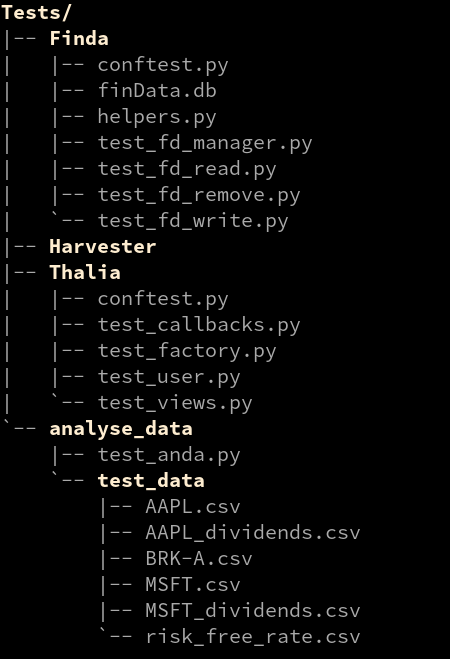
\includegraphics[scale=0.3]{06Testing/06Pictures/testingSuiteStructure.png}
   \caption{Tree of files in testing suite}
   \label{Testing Suite}
\end{figure}

\subsubsection{Unit Testing}
All team members were required to write automated unit tests for any code they wished to merge into the project’s master branch on GitHub. These were designed to test individual component modules and work independently from each other. The running of automated unit tests was performed by our CircleCI workflow. Although we are currently constrained by budget, in the future, our team plans on using the advanced metrics provided as part of CircleCI's paid plan to gain insight into how testing was performed throughout development. As part of the code review process, team members reviewed each other's tests as well as production code. This helped us to guarantee that unit tests were exhaustive and tested the full range of input classes and boundary cases for each software component. When designing these tests, team members also used white box testing techniques to maximize test coverage and make sure all possible paths of execution were accounted for.

In addition to uncovering bugs in our code, unit tests provided us with several other benefits. 
Firstly, we found that this strategy meshed well with our Agile approach to software development, as units of work loosely corresponding to functional requirements could be added to the live version of Thalia without the risk of breaking it. This, in turn, meant that after the continuous integration process was set up, we could continually test to see that all of our project's modules worked properly with each other. Since each functional requirement had an associated suite of unit tests, we could be reasonably certain that it was implemented correctly and would not block our progress down the line. 
In addition, team members could work on Thalia’s components interchangeably, as per our management strategy, since any undesired side effects of one person’s changes would cause the tests to fail. 
Finally, unit tests helped us to identify bugs resulting from merge conflicts and in doing so helped keep the live version of Thalia bug-free. This was especially important as we we're aiming to merge as quickly and as often as possible, in line with our Agile approach.

\subsubsection{Integration Testing}
Equally important to the unit tests were our integration tests. As with unit testing, we used a mixture of white and black box testing techniques. The majority of integration testing was done upon first setting up the CI process as this was when the individual components of Thalia first had to interact with one another. Subsequently, as we added new features, additional testing was performed to make sure new dependencies between components were integrated properly. Integration tests also helped us to refactor existing code to work better with other modules, since designing integration tests before writing code helped highlight areas where components' interfaces differed.

\subsubsection{End-to-end Testing}
Finally, upon completion of the prototype, we conducted extensive end-to-end testing. We used these tests to help identify system dependencies and to check whether data integrity was maintained throughout execution. They were also key in conclusively evaluating the functionality of our system, as they tested it holistically with real-world data as input, which is as close to a real world environment as we could get before the Alpha release.

\subsubsection{Data Harvester Logs}
Since our data is collected from 3rd party APIs, we opted to implement a series of logs to track their behaviour at runtime. These aim to record issues with received data that stop short of causing a catastrophic failure in the Data Harvester's execution. Such a situation might occur if an API were to change its policy or experience downtime, or if there is a problem with the network on Thalia's side. In this case, we are able to look through the logs and determine what caused the error and, consequently, what parts of the Data Harvester may need modification.

The logs record where and when data retrieval failed, what data was successfully retrieved and whether the data was successfully written to the database. In addition, they perform checks at runtime to test whether the API's data is of the expected type and format.

\begin{figure}[H]
   \centering
   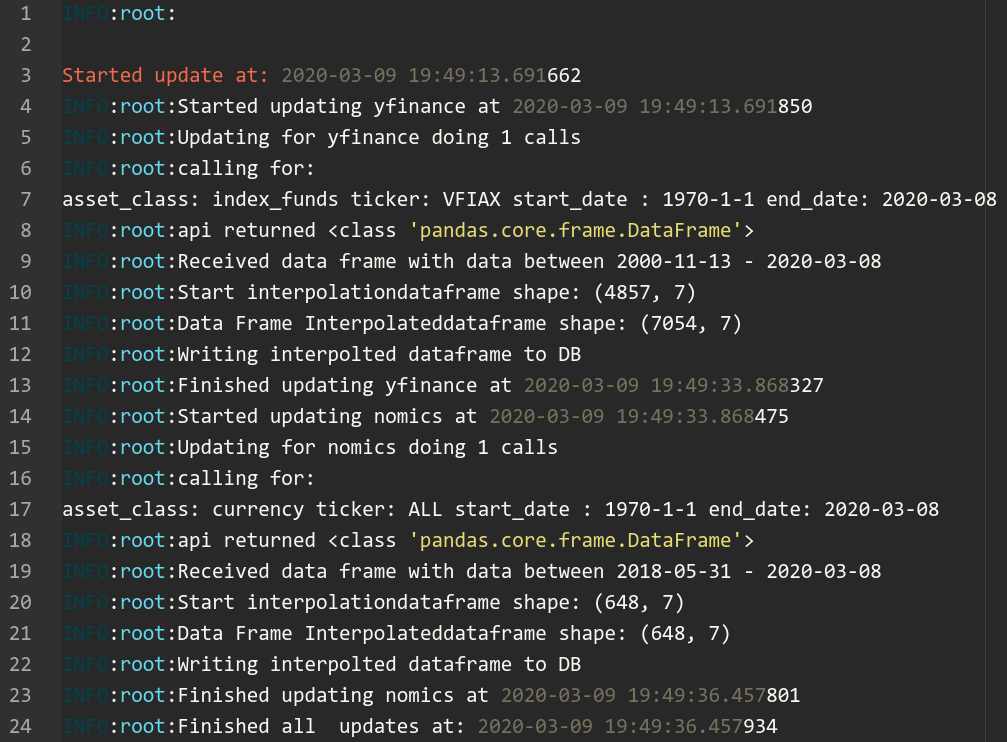
\includegraphics[scale=0.3]{06Testing/06Pictures/harversterLogEx.png}
   \caption{Example of data logged by harvester}
   \label{Example log}
\end{figure}

\subsection{Testing Tools}
The following is the list of 3rd party tools used by our testing suite to aid with the testing of Thalia and its components:

\begin{enumerate}
\item \textbf{Pytest:}
For our testing harness, we opted to use the standard python testing framework Pytest. With it we could easily create a testing suite independent of production code. By using simple assert statements Pytest remains easy to use, helping to reduce overhead for our team, most of whom had little to no experience writing automated tests for their code. Although simple, Pytest offers several powerful features that helped us during testing:

\begin{itemize}
\item Detailed introspection of failing tests helped decrease time spent debugging
\item Fixtures allowed us to automate test setup and teardown
\item Test discovery helped to keep the structure of the testing suite simple and physically separated from production code
\item Testing for expected exceptions allowed us to properly test for unexpected flows of events
\end{itemize}


\begin{figure}[H]
   \centering
   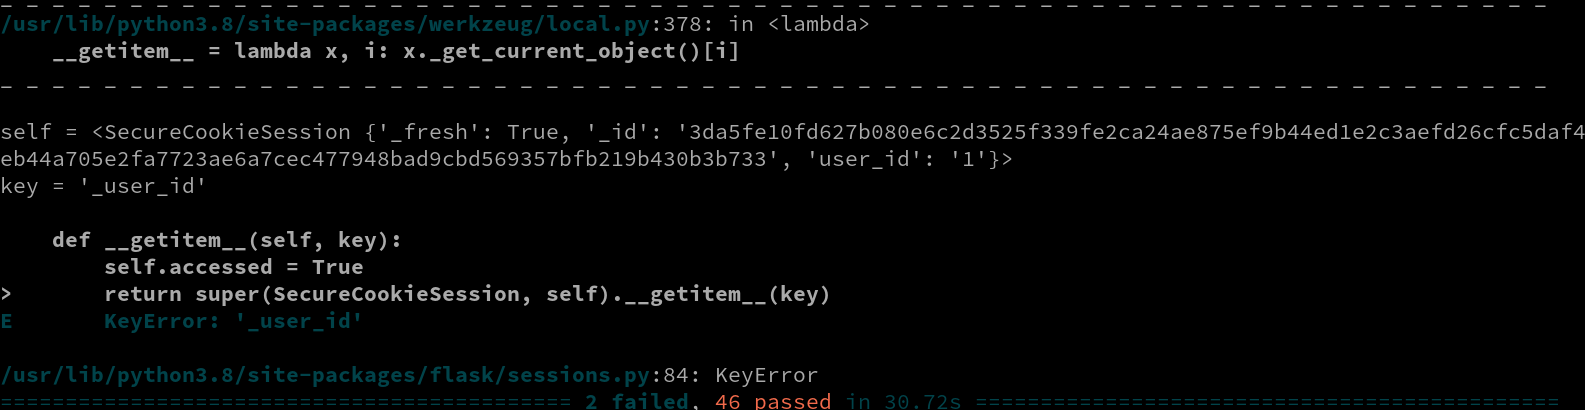
\includegraphics[scale=0.3]{06Testing/06Pictures/failedTest.png}
   \caption{Example of pytest assertion introspection}
   \label{Pytest example}
\end{figure}

\item \textbf{Mock:}
The Mock\cite{mock} package allowed us to replace parts of the system with mock objects. This was useful when testing API’s as it allowed us to control the input to the data harvester and allowed for repeatable execution and predictable output.

\item \textbf{Selenium}
Selenium\cite{selenium} is a testing tool we used to create unit and integration tests for Thalia’s website. Using Firefox or Chromium in headless or full browser mode it allowed us to automate user tasks such as clicking links and input. With it we were able to test logging in, running a simulation, registering a new account, and accessing the various pages of our website.

\item \textbf{Coverage:}
Coverage\cite{coverage} is a tool to measure code coverage in Python. It creates detailed reports on what lines of code are passed through during program execution. We used this in conjunction with Pytest to monitor what code was covered by tests to ensure our testing suite covered all possible branches of execution. In addition to validating test coverage, Coverage aided us in designing white-box tests by showing what parts of the codebase were in need of additional testing. Although not related to testing, the tool proved useful when refactoring code, as it allowed us to identify dead code.

\end{enumerate}


\subsection{Test Data}

We selected test data for our testing suite with the following considerations in mind:

\begin{itemize}

\item For black-box tests, the test data should contain representatives of all major equivalence classes of possible inputs.
\item For Black-Box tests, the test data should encompass all major boundaries of equivalence classes in the accepted inputs.
\item For White-Box testing, the data should be selected so tested code is executed exhaustively.

\end{itemize}

Broadly speaking, the data we used for testing can be separated into two categories, based on how it was collected. Either we wrote code to procedurally generate the data or we used a subsection of the real world data included in the final prototype and collected from financial data APIs. Each of these had its own benefits and drawbacks when being used to design tests.

\subsubsection{Mock Data}
In the real world, financial data, the prices of assets, tends to experience frequent and unpredictable fluctuations. Part of our testing strategy was the generation mock sets of historical price data that we designed to be as clean and easy to understand as possible. This allowed us to work with neat, easily understandable datasets. For example, we created a fictitious asset whose price increased linearly over time, an asset whose price decreased and an asset whose price remained fixed. All mock data was either generated procedurally by auxiliary code we wrote ourselves or hand-coded in cases where large amounts of data were not necessary (for example when testing the functionality of the database adapter). Being able to design these custom data sets helped us to overcome the following difficulties when designing and writing tests:

\begin{itemize}

\item Predictability:
Since complex financial equations are a key part of our service, a core requirement for our testing strategy was to be able to independently verify the results generated the Anda library. Having simple data showing, for example, a linear or quadratic increase in the daily price of an asset meant we could predict the expected results and compare them to Anda’s output. With real-world data, calculating expected values by hand would have been effectively impossible.

\item Interpretation of results:
Components of both Thalia Web and Finda modify financial data as it passes through them. It proved difficult to see the effect processing had on real-world data. Using clean datasets meant that the effect methods had on data could be examined by a human. This was a significant aid to development and saved us considerable time in the long run.

\item Designing tests:
When designing black-box tests for Thalia’s components, it was helpful to be able to create datasets that had specific properties for use as edge cases. A good example of this would be creating a series of prices that never decreased, as this represents an edge case for the calculation of an assets maximum draw-down.
\end{itemize}

\subsubsection{Real-world testing data}

In addition to generating our own assets for testing, we used a limited subset of real-world data for testing across components. We chose to include assets from across all supported asset classes over a significant period of time (several years as the simulation will at most span several decades). We found that this approach was easier than trying to emulate the complex fluctuations of real-world asset prices ourselves. While predicting the expected output of methods when handling real-world data was more difficult, we still found it proved useful in the following circumstances: 

\begin{itemize}

\item Validation:
Correct behaviour of system can be better confirmed after running them on real data \cite{liveData}. In our case, this is especially true since the data we work with is so complex.

\item Performance:
Performance of some of Thalia's features might vary based on the complexity of the input. As a result of this, real data was needed to properly assess performance.

\item Design:
An important design consideration was how clear the UI elements, especially the ones displaying data visually (for example the price graph) looked on screens of varying form factors. Having realistic test data helped us to better assess the quality of the user experience.

\end{itemize}
 

\subsection{Testing Results}

With all unit, integration and end to end tests passing, it is safe to assume that the core functionality of Thalia works as expected (short of a manageable risk of further bugs appearing, as no testing suite of this scale is perfect). Our unit tests are exhaustive, testing for the majority of possible edge cases and achieving a high level of coverage for each module tested. The functionality of the final prototype was additionally tested by hand and found to be working for the included data (a range of assets from all major asset classes with over 10 years of historical data). As such, it is safe to assume adding additional structurally similar data will not break the product.
At the time of writing, we deem the testing of Thalia to be successful and to have demonstrated the suitability of our product for further development and, eventually, bringing it to market. Going forward, we would like to implement a test driven development approach with the hopes of further reducing software defects and  improving quality of design\cite{TDD}.


\end{document}
